\section{Turbopompa}
\label{sec:turbopompa}

\subsection{Descrizione generica Mark 10}
\label{subsec:descrizione mark 10}

Il gruppo turbopompa Mark 10 è montato parallelamente alla mezzeria longitudinale della camera di spinta ed è sostenuto principalmente da due gruppi stabilizzatori a tre gambe saldati al corpo della camera e dai quattro condotti del propellente ad alta pressione installati tra la turbopompa e la camera di spinta. 
Il gruppo è composto da due pompe centrifughe montate schiena contro schiena (back-to-back) su un albero comune e azionate direttamente da una turbina a gas ad impulso.
L'albero principale e i componenti rotanti sono collegati direttamente all'albero e sono bilanciati dinamicamente.
L'albero è supportato da due gruppi di cuscinetti a sfere riscaldati elettricamente e raffreddati a carburante nell'area della pompa del LOX (per mantere l'ossigeno in fase liquid)e da un gruppo di cuscinetti a rulli raffreddati a carburante nell'area della turbina, mentre per isolare i propellenti, il fluido di raffreddamento e i gas caldi sono presenti un insieme di guarnizioni in carbonio, plastica (Kel-F, Teflon) e gomma sintetica (Buna-N, Viton-A).

\subsubsection{Pompe LOX e RP1}

L'esigenza di un sistema a turbopompa in uno stadio di lanciatore nasce quando il lanciatore stesso ha degli elevati requisiti di missione quali furono quelli dello stadio SI-C (e come la grande maggioranza dei primi e secondi stadi dei principali lanciatori odierni). Un sistema a serbatoio pressurizzato, per l'alimentazione dei 5 motori, dovrebbe essere progettato a sostenere elevate pressioni e quindi con un elevato spessore delle pareti dei tank. Introducendo il sistema di alimentazione a turbopompa, a patto di dimensionarlo correttamente, permette di diminuire il materiale per costruire i grandi tank di un sistema di queste dimensioni.
Tuttavia, un sistema cosi complesso introduce ulteriore complessità al progetto. Lo sviluppo moderno di tali sistemi prevede studi prelimiari con delle tecniche assodate da anni, come tabelle di valori specifici per le varie esigenze, con dati raccolti durante tutti gli anni di sviluppo. Al giorno d'oggi si conclude e si implementa la progettazione teorica tramite uno studio a CFD che tuttavia non verrà trattato in queste pagine. 

L’F-1 è dotato di due pompe del sitema Mark 10 di tipo centrifugo, una per l’ossidante e il combustibile; questa tipologia permette di ottenere un salto di pressione $\Delta P$ maggiore per singolo stadio (rotore + statore) rispetto alle pompe assiali a discapito di un leggero decremento dell’efficienza. Infatti, si è soliti usare pompe assiali solo laddove sono richiesti più stadi per ottenere un dato incremento di pressione come nel caso di LH2 dove a causa della bassa densità, il $\Delta P$ risulta limitato dalla massima velocità raggiungibile dai rotori.  Per pompe con fluido di lavoro a densità simile, come RP-1 e LOX, e simili pressione di scarico, si può mantenere la velocità angolare costante. 
Il progetto di una turbopompa ricerca principalmente la massimizzazione della velocità operativa poiché questo permette di ridurre le dimensioni della pompa stessa e di conseguenza il suo peso. Tuttavia, possibili effetti di cavitazione all’ingresso della pompa e sforzi dovuti alla forza centrifuga, vistosi nell’impeller (girante) e nella turbina, impongono un limite massimo alla velocità raggiungibile nelle zone periferiche dei componenti.

%Un primo obiettivo nella progettazione della pompa è quello di %massimizzare la velocità operativa. In questo modo vengono %ridotte le dimensioni della stessa e di conseguenza il peso. Il %limite massimo giri al minuto non deve superare un limite %massimo per evitare cavitazione e sforzi centrifughi. 

\subsubsection{Analisi pompa LOX}
\rfig{OXIDIZER_PUMP}{Prospettiva e dettagli pompa LOX}{OXIDIZER_PUMP}{0.5}
Nei seguenti paragrafi verrà considerato il funzionamento a regime, in particolare si vuole proporre un'analisi della pompa LOX del sistema di interesse. Partendo da diverse ipotesi e alcuni dati trovati sui principali manuali di interesse (NASA design Criteria - TURBOPUMPS for LRE e Centrifugal pumps for LRE), verranno costruiti i triangoli di velocità di impeller e inducer. Si verificherà la loro sensatezza tramite un controllo in termini di salto entalpico prodotto. Nel processo di analisi si cercherà di dare una spiegazione dei vari componenti. Infine, tramite un programma MATLAB e la libreria CoolProp si cercherà di dare un'analisi più accurata producendo anche un diagramma dell'impeller del LOX e quindi avere un primo ingombro radiale. 


%Criteri di progetto pompa
Per permettere al motore di generare la spinta per cui è stato progettato, la pompa deve essere in grado di fornire un adeguato valore di ‘prevalenza della pompa’ ed elaborare allo stesso tempo la portata volumetrica richiesta. Per la performance nel caso della pompa, al posto dell’incremento di pressione, è comune infatti usare il valore di prevalenza - headrise $H$- definito come l’altezza a cui può essere sollevato 1 kg di fluido con il lavoro compiuto idealmente per unità di massa dalla pompa. Si può usare la seguente formula per ricavarne il valore:
\begin{empheq}{equation*}
H = \frac{\Delta h_s}{g} = \int_{P_1}^{P_2} \frac{dp}{\rho g}
\end{empheq}

$\Delta h_s$ è direttamente legata al lavoro della pompa, rappresenta l'entalpia specifica del fluido di lavoro, e anche nel caso di fluido con elevata comprimibilità si può sempre scrivere
\begin{empheq}{equation*}
\frac{Lavoro}{Massa} = {\Delta h_s} = \frac{g H}{\eta_P}
\end{empheq}
dove con $\eta_P$ si intende il rendimento della pompa.
La prevalenza della pompa è inoltre direttamente proporzionale alla velocità periferica del disco della girante e da una prima osservazione si nota che il fluido viene introdotto assialmente vicino al mozzo della girante, senza alcun momento angolare, e viene rilasciato con una velocità tangenziale dipendente da $\beta_2$ angolo di back-leaning della palettatura e $v_{r2}$ velocità radiale di uscita del flusso. Quest’ultimo termine è legato alla portata volumetrica Q della pompa, ulteriore requisito di progetto, che essa deve essere in grado di soddisfare e che viene principalmente dettata dalle condizioni presenti in camera di combustione e al gas generator, più eventuali perdite di carico stimate lungo i tubi. 
Dal bilancio del momento della quantità di moto è possibile ricavare la coppia necessaria a mantenere il moto della girante e risalire perciò alla potenza:
\begin{empheq}{gather*}
P = \dot{m}{(\omega R_2 )}^2{(1 - {\frac{v_{r2}}{\omega R_2}} {\tan \beta_2})} = \dot{m}\frac{g H}{\eta_P}
\end{empheq}

Al valore di potenza è legato il termine $\psi$ coefficiente di prevalenza -head coefficient- della pompa
\begin{empheq}{gather*}
\psi = \eta_P {(1 - {\frac{v_{r2}}{\omega R_2}} {\tan \beta_2})} = \frac {g H}{{(\omega R_2 )}^2}
\end{empheq}
e per un design ottimale di pompa centrifuga deve essere contenuto tra 0.2 e 0.8. Valori maggiori dell’unità sono indicativi di palette realizzate per impartire in avanti il flusso e il $\Delta P$ tenderebbe ad aumentare all’aumentare della portata portando ad una generale instabilità del sistema di pressurizzazione.

Parametri adimensionali\\
La pompa è progettata, come detto precedentemente, per fornire una specifica prevalenza e portata volumetrica. Queste due quantità vengono usate per ricavare due parametri adimensionali
\begin{empheq}{gather*}
\text{Diametro specifico}\hspace{3pt}  d_s = \frac{D{(g H)}^\frac{1}{4}}{Q^\frac{1}{2}}         \qquad 
\text{Velocità specifica}\hspace{3pt}    n_s = \frac{\omega Q^\frac{1}{2}}{{(gH)}^\frac{3}{4}} 
\end{empheq}

Si verifica facilmente che il prodotto dei due parametri $n_s d_s = {2}/{\sqrt\psi}$  e poiché le pompe centrifughe, per costruzione, hanno un coefficiente di prevalenza $\psi$ minore dell’unità allora $n_s d_s > 2$. Diagrammi empirici nel piano $n_s, d_s$ permettono di fare considerazioni sulle prestazioni delle pompe e l’individuazione di zone ottimali di funzionamento a regime tenendo anche conto, solo ad un livello semplificato e non perfettamente realistico, di eventuali tolleranze di costruzione e rugosità interne che potranno poi essere modificate dopo prove al banco.

Sono forniti i seguenti requisiti costruttivi della pompa
\begin{table}[H]
\centering
\begin{tabular}{|c|c|c|c|c|c|c|}
\hline
$\bm{\eta_P \, [-]}$ & $\bm{P_ {TOT1} \, [Pa]}$ & $\bm{P_{TOT2} \, [Pa]}$ & $\bm{\rho [kg/m^3]}$ & $\bm{Q \, [m^3/s]}$ & $\bm{D_2 \, [m]}$ & $\bm{\omega \, [rad/s]}$  \\
\hline
$0.746$ & $448159$ & $1.1045e+7$ &  $1141$ & $1.5898$ & $0.4953$ & $575.12$  \\
\hline
\end{tabular}

\caption{Requisiti del sistema pompa LOX}
\label{table:LOX pump specs}

\end{table}

 da cui si ricavano i principali parametri prestazionali caratterizzanti la pompa in esame (il codice MATLAB con il dettaglio di tutti i conti eseguiti è riportato in appendice)

\begin{table}[H]
\centering
\begin{tabular}{|c|c|c|c|c|c|c|}
\hline
$\bm{H \, [m]}$ & $\bm{\Delta h_s \, [J/kg]}$ & $\bm{\psi \, [-]}$ & $\bm{P [W]}$ & $\bm{d_s \, [-]}$ & $\bm{n_s \, [-]}$ & $\bm{n_s d_s \, [-]}$  \\
\hline
$944.7827$ & $1.2424e+04$ & $0.4569$ &  $2.2440e+07$ & $3.8543$ & $0.7677$ & $2.9588$  \\
\hline
\end{tabular}

\caption{Parametri prestazionali del sistema pompa LOX}
\label{table:LOX pump performance}

\end{table}

Il punto di partenza nella progettazione della pompa è la scelta di un valore ottimale di velocità specifica $N_s$, definita in condizioni di design in relazione al numero di giri al minuto $N$ prestabiliti in condizioni stazionarie 
\begin{empheq}{equation*}
N_s = \frac{N\sqrt{Q}}{\Delta H^{0.75}}
\end{empheq}
questo primo valore permette di effettuare una prima selezione tra le varie tipologia di pompe (in particolare forma e tipologia di impeller) esistenti per concentrare lo studio su quella che meglio si potrebbe adattare ai requisiti del motore. Dal momento che sono noti i valori di portata e salto di pressione richiesto, viene ipotizzato un numero di giri al minuto $N$ per cominciare l'analisi.
 \\

Analisi Inducer\\
è la prima interfaccia tra il fluido di lavoro e il sistema pompa e deve essere progettata con l’intento di evitare il più possibile eventuali fenomeni di cavitazione che portano ad un grande degrado delle prestazioni generali. Il rischio di cavitazione è alto soprattutto nella zona di ingresso -inlet- della pompa dove il fluido di lavoro alla pressione più bassa che si riscontra in questa parte del ciclo, dovendo ancora cominciare la pressurizzazione, viene compresso grazie ai contributi di aumento di velocità radiale e velocità di rotazione della palettatura. Per caratterizzare la condizione di cavitazione bisogna introdurre una nuova grandezza, detta NPSH (Net Positive Suction Head), è un indice di merito della pressione in ingresso alla pompa. In particolare:
\begin{empheq}{equation*}
\left(NPSH\right) = \frac{P_{TOT1} - P_{vap}}{\rho g} 
\end{empheq}
In fase di progettazione si utilizza il parametro $\left( NPSH \right)_c$ come pressione critica all'ingresso per non avere cavitazione, valore determinato dal design globale del motore, ed è necessario che sia verificata la relazione $\left( NPSH \right)_a > \left( NPSH \right)_c $. 
In aggiunta per comparare le caratteristiche di aspirazione tra differenti geometrie e organizzazioni del sistema pompa si utilizza un parametro derivante direttamente dalla velocità specifica$N_s$ definita sopra, la suction specific velocity $N_{ss}$ e definita come segue.
\begin{empheq}{equation*}
N_{ss} = \frac{N\sqrt{Q}}{\left( NPSH \right)_c^{0.75}}
\end{empheq}
Alti valore di $N_{ss}$ sono indicativi della presenza di un inducer, a monte dell'impeller. Questo contribuisce attivamente a migliorare la prestazione globale della pompa dal momento che in questo modo si amplia il range di velocita rotazionali ammissibili senza incorrere nella cavitazione, fatto che permette una diretta riduzione del peso della pompa a parita di livello di potenza e prevalenza fornito al fluido.\\
\'E ora possibile andare a calcolare le velocità in ingresso, sezione 0, e in uscita, sezione 1, dall'inducer della pompa. Si effettua una ragionevole ipotesi sul 
valore del coefficiente di prevalenza $\psi_{ind}$, pari a $0.06$, relativo al solo tratto iniziale e basato su considerazioni tratte dal manuale NASA Design of LPRE; da questo dato si trovano in cascata la velocita di rotazione riferita al valore medio del raggio della palettatura inducer e i relativi diametri effettivi della palettatura e dell'albero motore sezioni 0 e 1. Dalla conoscenza del valore di portata volumetrica all'ingresso dell'inducer, leggermente maggiore di quello presente nel corpo impeller per tenere conto di eventuali perdite, si sfrutta l'equazione di continuità per ricavare i vettori velocità nel sistema di riferimento assoluto e solidale con il case della pompa. Tali velocità sono indicate con $\overrightarrow{c_0} e \overrightarrow{c_1}$ , rispettivamente per inlet e outlet inducer, e sono costituite da $c_u$ per indicare la componente tangenziale della velocità assoluta e da $c_m$ per riferirsi alla velocità meridionale, ovvero la componente della velocità assoluta che appartiene al piano radiale e assiale. Sono anche noti i valori di $\overrightarrow{u}$, vettore velocità periferica media di rotazione della palettatura nelle sezione di ingresso e uscita, dal momento che si sono ricavati i diametri effettivi e si conosce il numero di giri al minuti effettuati. Usando le relazioni trigonometriche, e la conservzione della componente meridionale della velocità tra la velocità assoluta $\overrightarrow{c}$ e la velocità espressa nel sistema di riferimento relativo e solidale con la palettatura in rotazione $\overrightarrow{v}$, si trova l'ultimo vettore necessario per andare a comporre il triangolo di velocità complessivo e determinare infine gli angoli di orientazione $\beta$ riferito all'inclinazione di  $\overrightarrow{v}$ e $\alpha$ riferito invece all'orientazione di $\overrightarrow{c}$.

Con le stesse relazioni sopra descritte, è anche possibile andare a trovare la velocità all'estremo superiore -tip- della paletta per valutare un ulteriore parametro di progetto, la -vane solidity tip-; essa è definita come la sezione anulare normale alla direzione della velocità assiale di effettivo passaggio del fluido di lavoro.
\\

Analisi Impeller\\
Bisogna anche in questo fare riferimento ad una ragionevole ipotesi sulla perdita di prevalenza $H$ nella sezione anulare di passaggio del fluido a causa di attriti e conseguente dissipazione di energia, dal manuale risulta $H_e = 0.3H$ come termine di perdita. A questo punto è possibile calcolare la prevalenza effettiva fornita della sezione della girante -impeller- e sono noti inoltre il diametro nella sezione 1 -outlet inducer/inlet impeller- e nella sezione 2 -outlet impeller-. Con un ragionamento del tutto analogo a quello relativo all'inducer è possibile costruire il triangolo di velocità dato dalla composizione della velocità assoluta  $\overrightarrow{c}$, della velocità relativa $\overrightarrow{v}$, con i rispettivi angoli di orientazione $\alpha$ e $\beta$ e della velocità periferica media di rotazione $\overrightarrow{u}$. Per i procedimenti di analisi della conservazione della portata e di calcolo effettivo mediante relazioni trigonometriche passo per passo si rimanda al codice matlab $POMPA_{LOX}$ allegato in appendice.
\\

Analisi casing pompa: vani diffusori\\
Il principale compito del casing è quello di convertire l'elevata energia cinetica del fluido di lavoro in uscita dalla sezione 2 dell'impeller in pressione statica; questo elemento non contribuisce quindi in alcun modo alla generazione di un valore di prevalenza. Il casing può essere formalmente diviso in due sezioni: una frontale nominata -suction nozzle- con il compito di convogliare debitamente il flusso nella sezione di uscita -volute / (voluta in italiano)- che invece si occupa della effettiva conversione energetica. La sezione frontale ha una lughezza ridotta per cercare di limitare al minimo le perdite di pressione per attrito contro le pareti rigide. Con i dati in possesso si procede al dimensionamento di un casing con geometria double-volute ($180\degree$) e singola sezione di efflusso per il flusso.\\
Per calcolare la velocità media del flusso all'interno della voluta si assume come riferimento un parametro $K_v$ determinato sperimentalemente tramite prove al banco di differenti tipologie di vani diffusori. Per i calcoli $K_v = 0.337$ da manuale.
\begin{empheq}{equation*}
c_3 = K_v \sqrt{2 g H}
\end{empheq}
Si procede al calcolo dell'area del tratto divergente della voluta, imponendo per ciascuna sezione un valore di $\alpha_{volute}$ compreso tra $0\degree$ e $180\degree$. Nota la geometria e servendosi dell'equazione di continuità è infine possibile ricavare i valori di velocità assoluta relativi alla sezione di ingresso alla voluta e di efflusso finale per valutare il corretto funzionamento del sistema pompa e l'incremento di pressione statica che riesce ad imporre al fluido.

\begin{table}[H]
\centering
\begin{tabular}{|c|c|}
\hline
$\bm{v_{voluteIN} \, [m/s]}$ & $\bm{v_{voluteOUT} \, [m/s]}$  \\
\hline
$103.7019$ & $29.1447$   \\
\hline
\end{tabular}

\caption{Velocità efflusso del sistema pompa LOX: casing}
\label{table:LOX pump casing}

\end{table}

\subsubsection{Analisi pompa RP-1}
Si riportano i principali parametri di interesse calcolati con gli stessi procedimenti della pompa LOX.

\begin{table}[H]
\centering
\begin{tabular}{|c|c|c|c|c|c|c|}
\hline
$\bm{\eta_P \, [-]}$ & $\bm{P_ {TOT1} \, [Pa]}$ & $\bm{P_{TOT2} \, [Pa]}$ & $\bm{\rho [kg/m^3]}$ & $\bm{Q \, [m^3/s]}$ & $\bm{D_2 \, [m]}$ & $\bm{\omega \, [rad/s]}$  \\
\hline
$0.760$ & $310264$ & $1.2824e+7$ &  $808.9324$ & $0.9617$ & $0.59436$ & $574.020$  \\
\hline
\end{tabular}

\caption{Requisiti del sistema pompa RP-1}
\label{table:RP-1 pump specs}

\end{table}

\begin{table}[H]
\centering
\begin{tabular}{|c|c|c|c|c|c|c|}
\hline
$\bm{H \, [m]}$ & $\bm{\Delta h_s \, [J/kg]}$ & $\bm{\psi \, [-]}$ & $\bm{P [W]}$ & $\bm{d_s \, [-]}$ & $\bm{n_s \, [-]}$ & $\bm{n_s d_s \, [-]}$  \\
\hline
$1.5774e+03$ & $2.0361e+04$ & $0.5318$ &  $1.6218e+07$ & $6.7598$ & $0.4057$ & $2.7427$  \\
\hline
\end{tabular}

\caption{Parametri prestazionali del sistema pompa RP-1}
\label{table:RP-1 pump performance}

\end{table}

\begin{table}[H]
\centering
\begin{tabular}{|c|c|}
\hline
$\bm{v_{voluteIN} \, [m/s]}$ & $\bm{v_{voluteOUT} \, [m/s]]}$  \\
\hline
$153.7897$ & $31.7356$   \\
\hline
\end{tabular}

\caption{Velocità efflusso del sistema pompa RP-1: casing}
\label{table:RP-1 pump casing}

\end{table}



\subsection{Turbina}
\label{subsec:turbina}

\subsubsection{Descrizione turbina}

\rfig{turbina_general}{Turbina ad impulso VC dell'F-1}{turbina_general}{0.45}

La turbina che fornisce la potenza necessaria alle pompe del sistema motore F-1 è definita come turbina a impulso (variazione di pressione statica solamente negli statori), e cosiddetta 2 row - velocity compounded (VC). Ovvero costituita da 2 file di rotori intramezzati da uno statore. Il gas caldo prima di passare in questa zona viene espanso in una schiera di ugelli che aumentano notevolmente la velocità: per le turbina VC, idealmente, tutta l'espansione avviene in questa zona. Successivamente i rotori, venendo impattati da un gas, sottraggono quantità di moto al fluido. Lo statore intermedio ha la funzione di reinidirizzare il flusso all'ingresso dell'ultimo rotore. Oltre a queste zone citate, nella turbina c'è una zona di ingresso, manifold, che convoglia il flusso ai nozzles. I nozzles, che sono generalmente convergenti-divergenti per una turbina VC, espandono il gas e lo incurvano per affrontare il primo rotore. Entrambe le i rotori della turbina sono costituiti da dischi i quali presentano dei 'fir tree' slot lungo la circonferenza, dove vengono inserite e rivettate le palette. Il rotore iniziale è calettato direttamente sull'albero, l'ultimo viene imbullonato sul primo e vengono separati da un distanziale. Le guarnizioni sono di diverso tipo, in questa sede non verranno approfondite, ma hanno il compito di contenere le perdite e quindi migliorare l'efficienza. 

\subsubsection{Turbina - scelte progettuali}

Il sistema turbina di un endoreattore ha una vita breve ma è sottoposto a parecchi carichi critici. Il design deve essere compatto e leggero, il fluido che espande deve avere un alto contenuto energetico, il lavoro specifico in uscita deve essere alto. La progettazione dell'elemento turbina è direttamente collegato al tipo di ciclo di alimentazione del motore, nel caso di un GG si vuole massimizzare il salto di pressione per minimizzare la portata spillata prima della camera di spinta (questo infatti massimizza l'impulso specifico del sistema). 

Per l'analisi del percorso aerotermodinamico del gas si tratta un flusso di gas combusti a chimica congelata (FE). Tali parametri fisici sono stati interpolati tramite MATLAB da una tabella fornita dal libro [] (Modern engieering for LRE systems, AIAA, Huzel, ...), dati ricavati da test sperimentali di NASA. Di seguito vediamo quali parametri principali vengono utilizzati per la scelta e il dimensionamento della turbina. 

\begin{itemize}

\item
\textbf{Spouting velocity:} è la velocità teorica che il flusso di gas avrebbe se espandesse dalla pressione di ristagno alla pressione di uscita (data dal rapporto $\epsilon$ di espansione)
\begin{empheq}{gather*}
C_0 = \sqrt{2C_{p,gg}T_{in} \left(1 - \epsilon^\frac{1-\gamma }{\gamma}\right)}
\end{empheq}

\item
\textbf{Rapporto isoentropico delle velocità:} è il rapporto tra velocità tangenziale del disco rotorico e la spouting velocity.

\begin{empheq}{equation*}
\frac{U}{C_0} = 
\end{empheq}

\parbox[t]{\dimexpr\textwidth-\leftmargin}{%

\begin{wrapfigure}{r}{0.4\linewidth}
	\centering
	\vspace{-\baselineskip}
	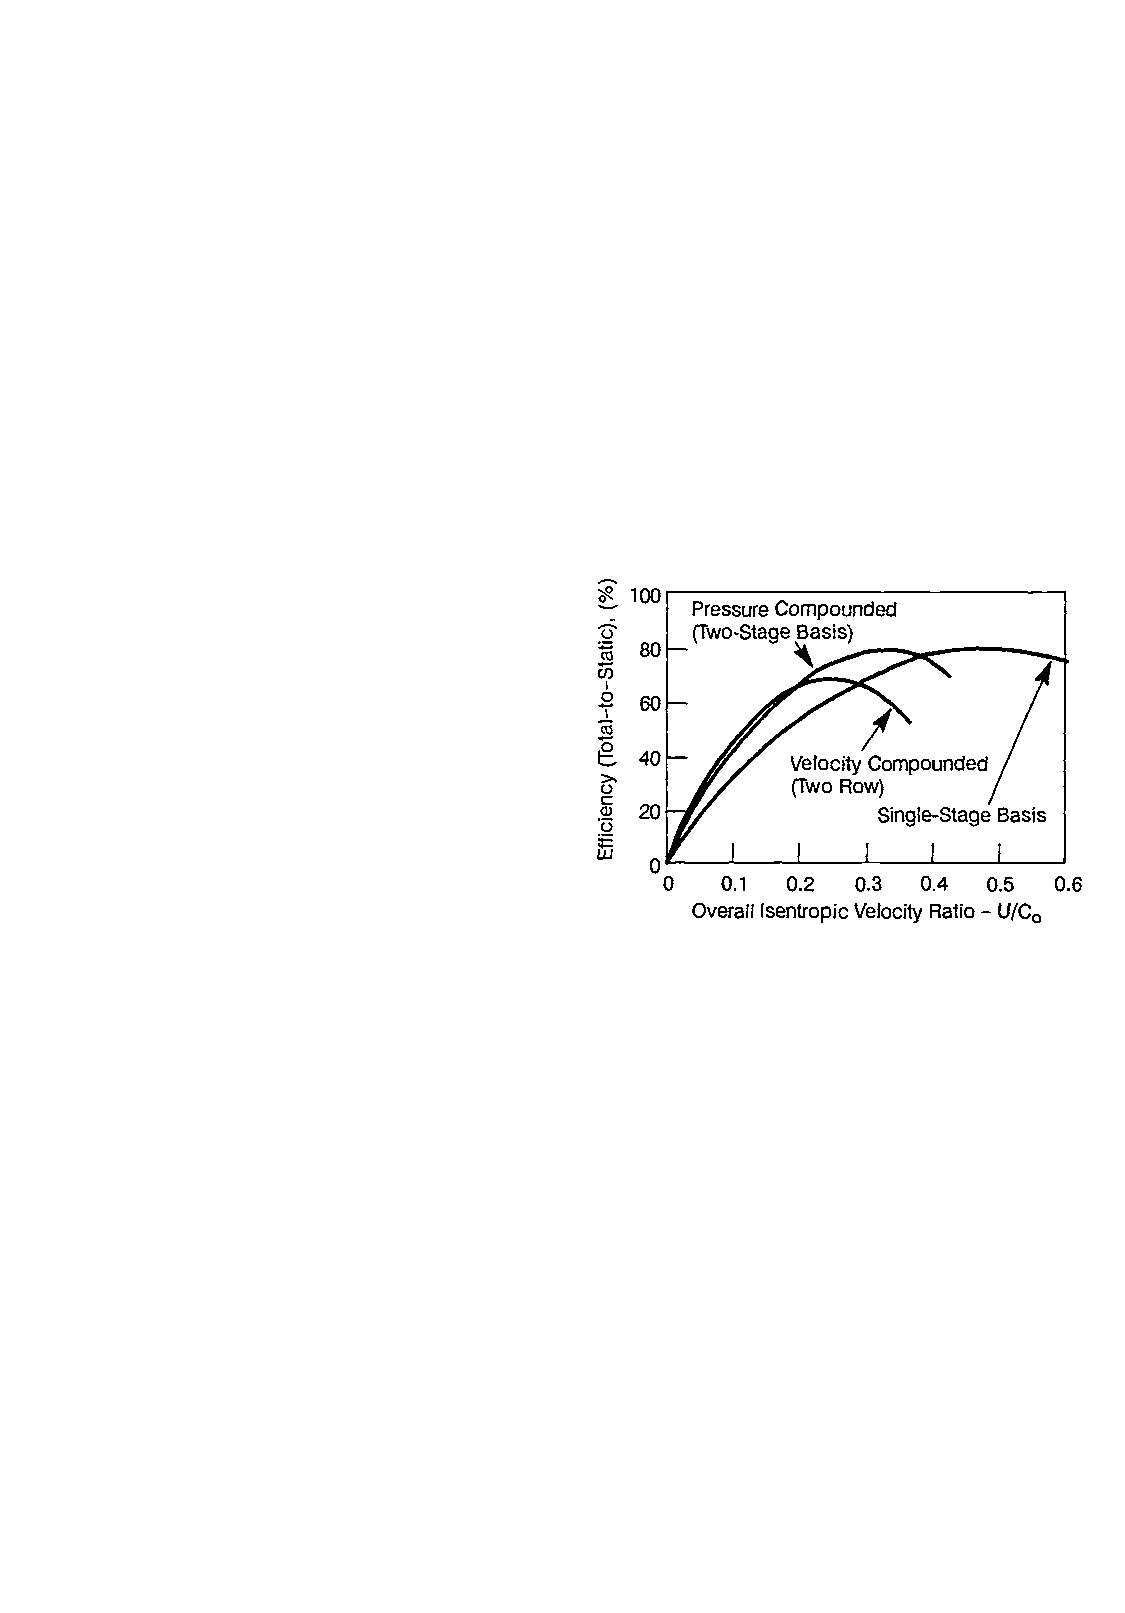
\includegraphics[width=\linewidth]{rendimenti_turbina}
	\caption{Rendimenti in funzione del rapporto di velocità}
	\label{fig:rendimenti_turbina}
\end{wrapfigure}

Questo valore è utile per capire la scelta progettuale effettuata per il tipo di turbina. Infatti, come già detto, nei cicli GG il salto di pressione in turbina è molto alto: questo implica un valore di $C_0$ elevato. Per avere una buona efficienza si possono percorrere più scelte progettuali (basandosi sul grafico x dei rendimenti). Si può scegliere di avere un alto rapporto di velocità con una singola ruota che 'assorba' tutta l'energia del flusso. Questo provocherebbe nel nostro caso una velocità di rotazione troppo elevata (quindi ingombro maggiore, inoltre la velocità di rotazione è fissata dalla pompa). Per usare altre turbine, cercando di avere un'alta efficienza si cerca di diminuire il rapporto di velocità aumentando gli stadi, ovvero la velocità del flusso è assorbita da più dischi che ruotano a velocità minori e sono più piccoli.

Le turbine PC (generano il salto di pressione in tutti gli statori) sono più efficienti ma più pesanti. Per cui si è optato per un sistema VC, che ha buona efficienza a bassi rapporti di velocità e permette un risparmio in peso.
}
\end{itemize}
\subsubsection{Analisi quantitativa - dimensionamento}

L'obiettivo ora è quello di cercare di dare un'idea a livello quantitativo dei vari componenti, generando un diagramma di velocità della turbina. 
Per questa sezione si sono presi in considerazione i requisti del sistema turbina, si sono ipotizzati diversi valori di rendimenti e sono state fatte alcune assunzioni ragionevoli per questo tipo di sistema (AIAA, modern engineering of LRE, Huzel ..). Abbiamo assunto i seguenti requisiti di sistema

\begin{table}[H]

\centering
\begin{tabular}{|c|c|c|c|c|c|}
\hline
$\bm{T_in \, [K]}$ & $\bm{p_in \, [bar]}$ & $\bm{\epsilon}$ &  $\bm{O/F}$ & $\bm{\dot{m} \, [kg/s]}$ & $\bm{\omega \, [rad/s]}$  \\
\hline
$1062$ & $67.57$ & $16.4$ &  $0.416$ & $75.75$ & $574.4$ \\
\hline
\end{tabular}

\caption{Requisiti del sistema turbina}
\label{table:turbine specs}

\end{table}

Assumendo tali dati, aggiungendo alcune ragionevoli ipotesi tratte dal libro AIAA e risolvendo il sistema di equazioni associato al problema, troviamo il seguente diagramma velocità e i corrispondenti valori di velocità e angoli. Si rimanda all'appendice per tutti i dettagli su ipotesi fatte, impostazione del sistema di equazioni e risoluzione del sistema tramite MATLAB.